\documentclass{ctexart}
\usepackage{amsmath}
\usepackage{float}
\usepackage{graphicx}
\usepackage{lmodern} % Latin Modern fonts, scalable
\usepackage[T1]{fontenc}
\usepackage[a4paper,left=25mm,right=25mm,top=31mm,bottom=31mm]{geometry}
\pagestyle{plain}
\graphicspath{{./images}}

\begin{document}

\begin{center}
    \LARGE \textbf{企业实习\;第九周实习报告}\\
    \vspace{10pt}
    \normalsize 小米自动驾驶与机器人部\;\;陈子林
\end{center}

\section{本周工作主要内容}

本周为小米实习第六周(8.18--8.22),主要围绕机器人仿真测试与控制算法验证开展了如下工作:

\begin{enumerate}
    \item 搭建并完善基于宇树 H1\_2 机器人与 G1 机器人的 Mujoco 仿真平台。  
    在此过程中,对通信链路进行了调试与验证,确保仿真环境中的数据输入、状态反馈和指令信号与真实机器人硬件环境保持一致,从而保证测试的连续性和可靠性。  
    
    \item 在搭建完成的仿真环境中开展上肢精度测试。  
    通过在不同运动姿态下对关节角度进行实时采集与比对,评估 Mujoco 仿真模型在执行指定运动轨迹时的精度与一致性,进一步验证仿真器的可用性与模型参数合理性。  
    
    \item 进行下蹲耐久测试的调试工作(仿真环境)。  
    构建并实现了一个简易控制器,使机器人能够在仿真环境中反复、连续完成下蹲动作。在施加 $100\sim150\text{N}$ 干扰力的情况下,机器人仍能保持姿态稳定,验证了控制器在基础抗扰性方面的有效性。  
    
    \item 编写相关技术文档并完善操作说明。  
    将搭建步骤、调试方法和测试结果进行系统化整理,编写成面向其他测试人员的操作手册,便于后续复现测试环境和快速定位问题。
\end{enumerate}

\begin{figure}[H]
      \centering
      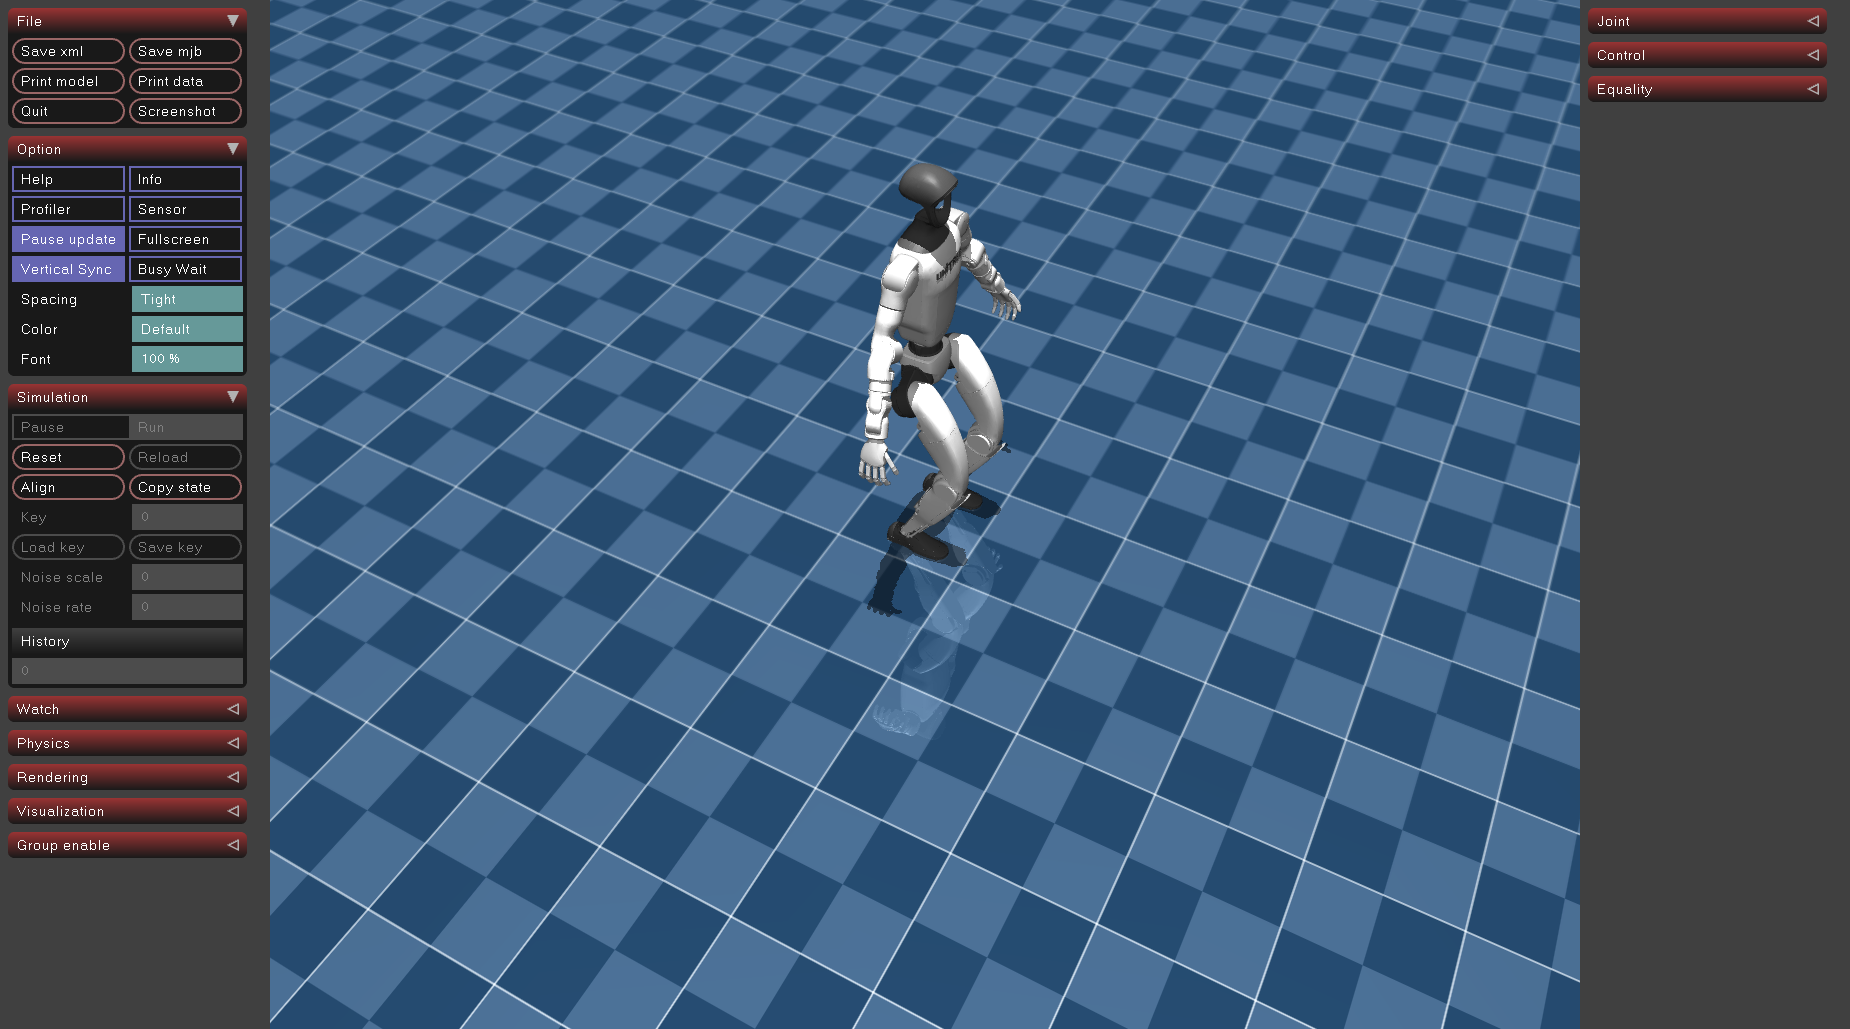
\includegraphics[width = 0.8\textwidth]{mujoco_visualize.png}
      \caption{Mujoco 仿真界面展示,验证机器人模型在虚拟环境下的运动表现}
\end{figure}

\begin{figure}[H]
      \centering
      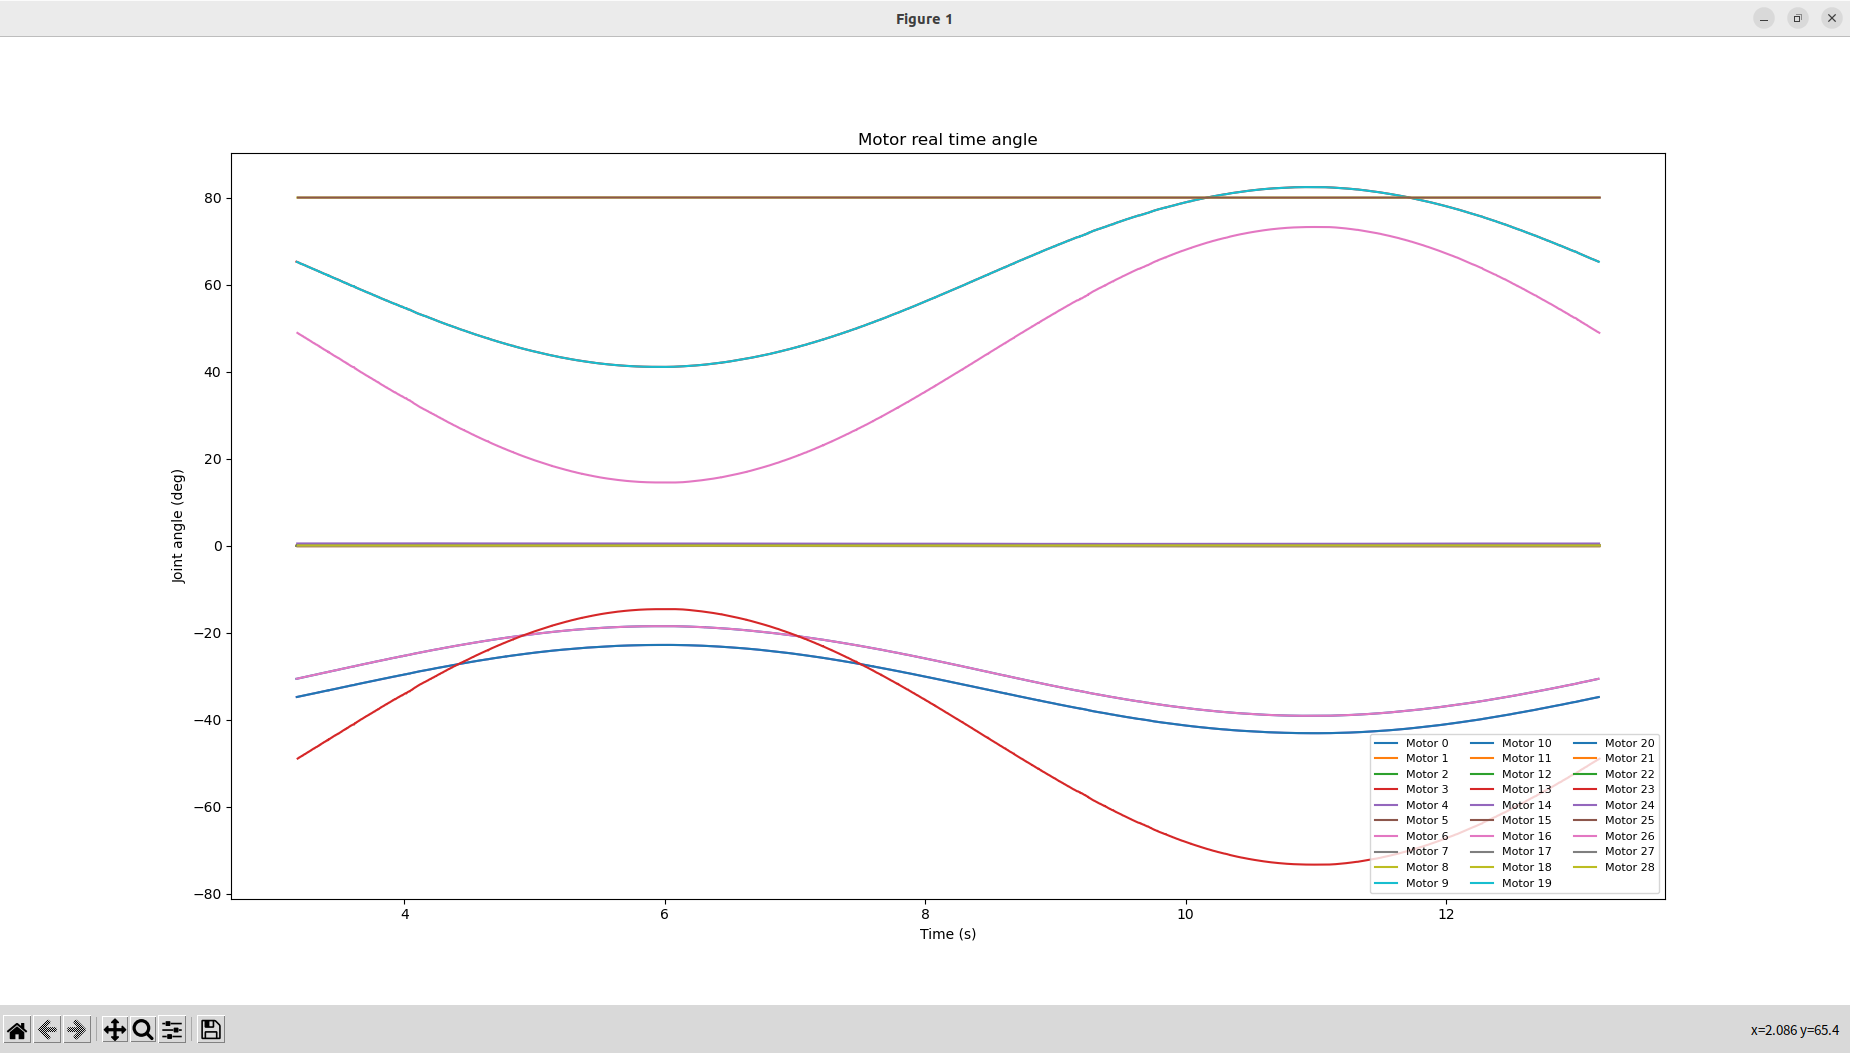
\includegraphics[width = 0.8\textwidth]{plotter.png}
      \caption{实时读取关节角度并绘制曲线用于精度检测}
\end{figure}

\section{后续工作计划}

基于当前项目进展和测试中发现的实际问题,下一阶段的工作将主要聚焦于以下关键目标:

\begin{enumerate}
    \item 将下蹲耐久测试迁移至真实机器人平台,验证仿真环境中控制算法与硬件平台的一致性,并进一步检验除上肢精度外的整体仿真器效果。  
    
    \item 优化控制算法的参数与策略。  
    在现有简易控制器的基础上,通过引入更合理的反馈机制或阻尼控制手段,提升机器人在受到更大外界扰动时的稳定性,确保在复杂环境下仍能保持不倒地。  
\end{enumerate}

\end{document}
